\documentclass[a4paper,12pt]{article}
\usepackage[table]{xcolor}
\usepackage{array,amsmath,amssymb,multicol,tikz}
\usepackage{hyperref,colonequals}
\usepackage[margin=2cm]{geometry}
\usepackage{fancyvrb}
\usetikzlibrary{calc,arrows.meta}
\usepackage{xcolor}

\tikzset{
arr/.style={line width=1pt,-{Straight Barb[width=6pt, length=3pt]}, shorten >=2pt}
}

\pagestyle{empty}

\newcommand\N{\mathbf{N}}
\newcommand\Q{\mathbf{Q}}
\newcommand\R{\mathbf{R}}
\newcommand\Z{\mathbf{Z}}

\newcommand\rem{\textup{rem}}

\setlength{\parindent}{0pt}

\begin{document}

\begin{center}
\parbox{3cm}{\flushleft\bf Discrete\linebreak Structures}
\hfill
\parbox{7cm}{\centering {\bf\Huge Samples, Part 3}}
\hfill
\parbox{3cm}{\flushright\bf Spring 2021 \linebreak May 28}
\end{center}

\hrule\vspace{2pt}\hrule

\hrule


\vspace{10pt}
{\bf Combinatorics.}

\begin{enumerate}
% 1.(a)
\item {\small \em Given a word problem, count variants using the product, sum, difference rules.}\\
The following problem deals with English alphabet consisting of exactly $26$ letters (assume that 
all letters are upper-case). Assume that there are $6$ vowels ({\tt A}, {\tt E}, {\tt I}, {\tt O}, {\tt U}, {\tt Y}); 
all the other $20$ letters are considered consonants. 
\begin{enumerate}
\item A car license number in some city should consist of $4$ different letters; it should start with 
two consonants followed by two vowels. How many license numbers are possible?
\item A car license number in some other city should consist of $4$ different letters; 
two consonants and two vowels (in any order). How many license numbers are possible?
\item A car license number in some other city should consist of $4$ letters \textendash{} not necessarily different; 
two consonants and two vowels (in any order). How many license numbers are possible?
\end{enumerate}


% 1.(b)
\item {\small \em Given a set of restrictions and symmetries, count variants using the division rule.}\\
Consider the following three situations and find the number of variants to complete each task:
\begin{enumerate}
\item In how many ways can we arrange $7$ bits in the following string: $\mathtt{0000111}$ (the order of bits matters; 
the string must contain four 0s and three 1s).
\item There are $7$ seats enumerated with numbers $1,2,\ldots,7$. In how many ways can we seat three people on these seats
(the only thing that matters is \textendash{} which seats are occupied; it does not matter who is seated where). 
\item A traveler needs to go from point $A$ to point $B$ in a city where there the streets are perpendicular and 
all blocks have square shape. He should go three blocks to the north and four blocks to the east (extra circling around is
not allowed). In how many ways can he pick a route that leads from $A$ to $B$ following these rules?
\begin{center}
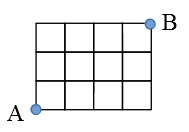
\includegraphics[width=1.2in]{figs/part3-square-city.png}
\end{center}
\end{enumerate}


% 1.(c)
\item {\small \em Count variants using combinations and permutation formulas with or without repetition.}\\
Assume that we have $4$ different sorts of candy (and any two pieces of the same sort of candy are considered indistinguishable).
We want to create a set of $7$ candies; and there are no limitations on how many candies of each sort should be in the set.
\begin{enumerate}
\item How many sets of $7$ candies can be created, if the order of candies in the set (which candy is the first, which 
is the second etc.) is important? 
\item How many sets of $7$ candies can be created, if the order of candies in the set does not matter?
\end{enumerate}


% 1.(d)
\item {\small \em Given a polynomial, find coefficients using binomial and multinomial rules.}\\
Consider the following expression ${\displaystyle \left(x^2 - \frac{1}{x}\right)^{9}}$. 
\begin{enumerate}
\item
How many terms are there in the expression  after we expand it using the binomial formula?
\item 
Which term has the largest (positive) coefficient; find that term.
\end{enumerate}
\end{enumerate}





\vspace{10pt}
{\bf Recurrent Sequences.}

\begin{enumerate}
%2.(a)
\item {\small \em Evaluate $\sum\limits_{i=0}^n \ldots$ and similar constructs.}\\
ABC

%2.(b)
\item {\small \em Prove a property of a recurrent sequence by induction or using invariants.}\\
ABC

%2.(c)
\item {\small \em Prove that a recurrent sequence has a closed formula using induction.}\\
ABC

%2.(d)
\item {\small \em Given a 1st order non-homogeneous recurrence, solve it.}\\
ABC

%2.(e)
\item {\small \em Given a 2nd order homogeneous recurrence, solve it.}\\
ABC

%2.(f)
\item {\small \em Given a word problem (sets of strings, Tower of Hanoi, tilings, etc.) build recurrences.}\\
ABC

%2.(g)
\item {\small \em Given a divide-and-conquer type recurrence, solve it with Master theorem.}\\
ABC
\end{enumerate}



\vspace{10pt}
{\bf Big-O notation.}


\begin{enumerate}
%3.(a)
\item {\small \em Given functions $f,g$, check by definition that $f(n)$ is in $O(g(n))$, $\Omega(g(n))$, $\Theta(g(n))$.}\\
ABC

%3.(b)
\item {\small \em Given a function $f(x)$, simplify it to get its ``optimal'' $O(g(x))$ or $\Theta(g(x))$ class.}\\
ABC

%3.(c)
\item {\small \em Given a collection of functions, arrange them by growth.}\\
ABC

%3.(d)
\item {\small \em Given a pseudocode, basic operations and input length, estimate its time as $O(g(n))$.}\\
ABC
\end{enumerate}



\end{document}
